\documentclass{standalone}
\usepackage{tikz}
\usepackage{ctex,siunitx}
\setCJKmainfont{Noto Serif CJK SC}
\usepackage{tkz-euclide}
\usepackage{amsmath}
\usetikzlibrary{patterns, calc,3d}
\usetikzlibrary {decorations.pathmorphing,decorations.pathreplacing,decorations.shapes}
\tikzset{label style/.append style={font=\small}}
\begin{document}
\small
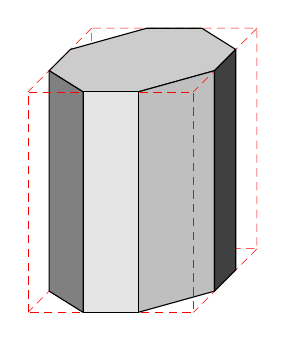
\begin{tikzpicture}[>=latex,scale=0.7]
  \draw[very thin,densely dashed,red](0,0,0)--(0,4,0)--(3,4,0)--(3,0,0)--cycle(0,4,0)--(0,4,3)(0,0,0)--(0,0,3);
  \draw[fill=gray!40,line join =round](0,4,1)--(0,4,2)--(1,4,3)--(2,4,3)--(3,4,2)--(3,4,1)--(2,4,0)--(1,4,0)--cycle;
  \draw[fill=gray,line join =round](0,4,2)--(0,0,2)--(1,0,3)--(1,4,3)--cycle;
  \draw[fill=lightgray,line join =round](2,4,3)--(2,0,3)--(3,0,2)--(3,4,2)--cycle;
  \draw[very thin,densely dashed,red](3,4,0)--(3,4,3)(3,0,0)--(3,0,3);
  \draw[fill=darkgray,line join =round](3,4,2)--(3,0,2)--(3,0,1)--(3,4,1)--cycle;
  \draw[very thin,densely dashed,red](0,0,3)--(0,4,3)--(3,4,3)--(3,0,3)--cycle;
  \draw[fill=lightgray!40,line join =round](1,4,3)--(1,0,3)--(2,0,3)--(2,4,3)--cycle;
\end{tikzpicture}
\end{document}